\documentclass[14pt, aspectratio=169]{beamer}

\usetheme{CambridgeUS}
\usecolortheme{dolphin}
\useinnertheme{rectangles}
\usepackage{svg}

\usepackage{multicol}
\usepackage[subpreambles=true]{standalone}
\usepackage{import}

\title{M.O.S.I.S Progress Report Presentation}
\author{Fabio J. Matos Nieves \& Eduardo S. Miranda Figueroa }
\institute{University of Puerto Rico Mayagüez Campus}
\date{September 28, 2023}

\begin{document}
\begin{frame}
	\maketitle
\end{frame}
\begin{frame}{Table of Contents}
	\begin{multicols}{2}
		\tableofcontents
	\end{multicols}
\end{frame}
\section{Introduction}
\subsection{Problem Statement}
\begin{frame}{Problem Statement}

\end{frame}
\subsection{Changes and Updates}
\begin{frame}{Changes and Updates}

\end{frame}
\section{Body}
\subsection{Design Alternatives}
\begin{frame}{Design Alternatives}
\end{frame}
\subsection{Analysis Criteria}
\begin{frame}{Analysis Criteria}

\end{frame}
\subsection{System Architecture}
\subsubsection{M.O.S.I.S Microscope}
\begin{frame}{Microscope Block Diagram}
	\begin{figure}
		\includesvg[inkscapelatex=false,height=0.7\textheight]{../../Progress_Report_Document/Appendix/System_Architecture_and_Interfaces/Hardware_Block_Diagram/Figures/hardware_block_diagram.svg}
		\caption{Microscope Block Diagram}
	\end{figure}

\end{frame}
\subsubsection{M.O.S.I.S UI 2.0}
\begin{frame}{M.O.S.I.S UI 2.0: Mock-ups (Main Menu)}
	\begin{figure}
		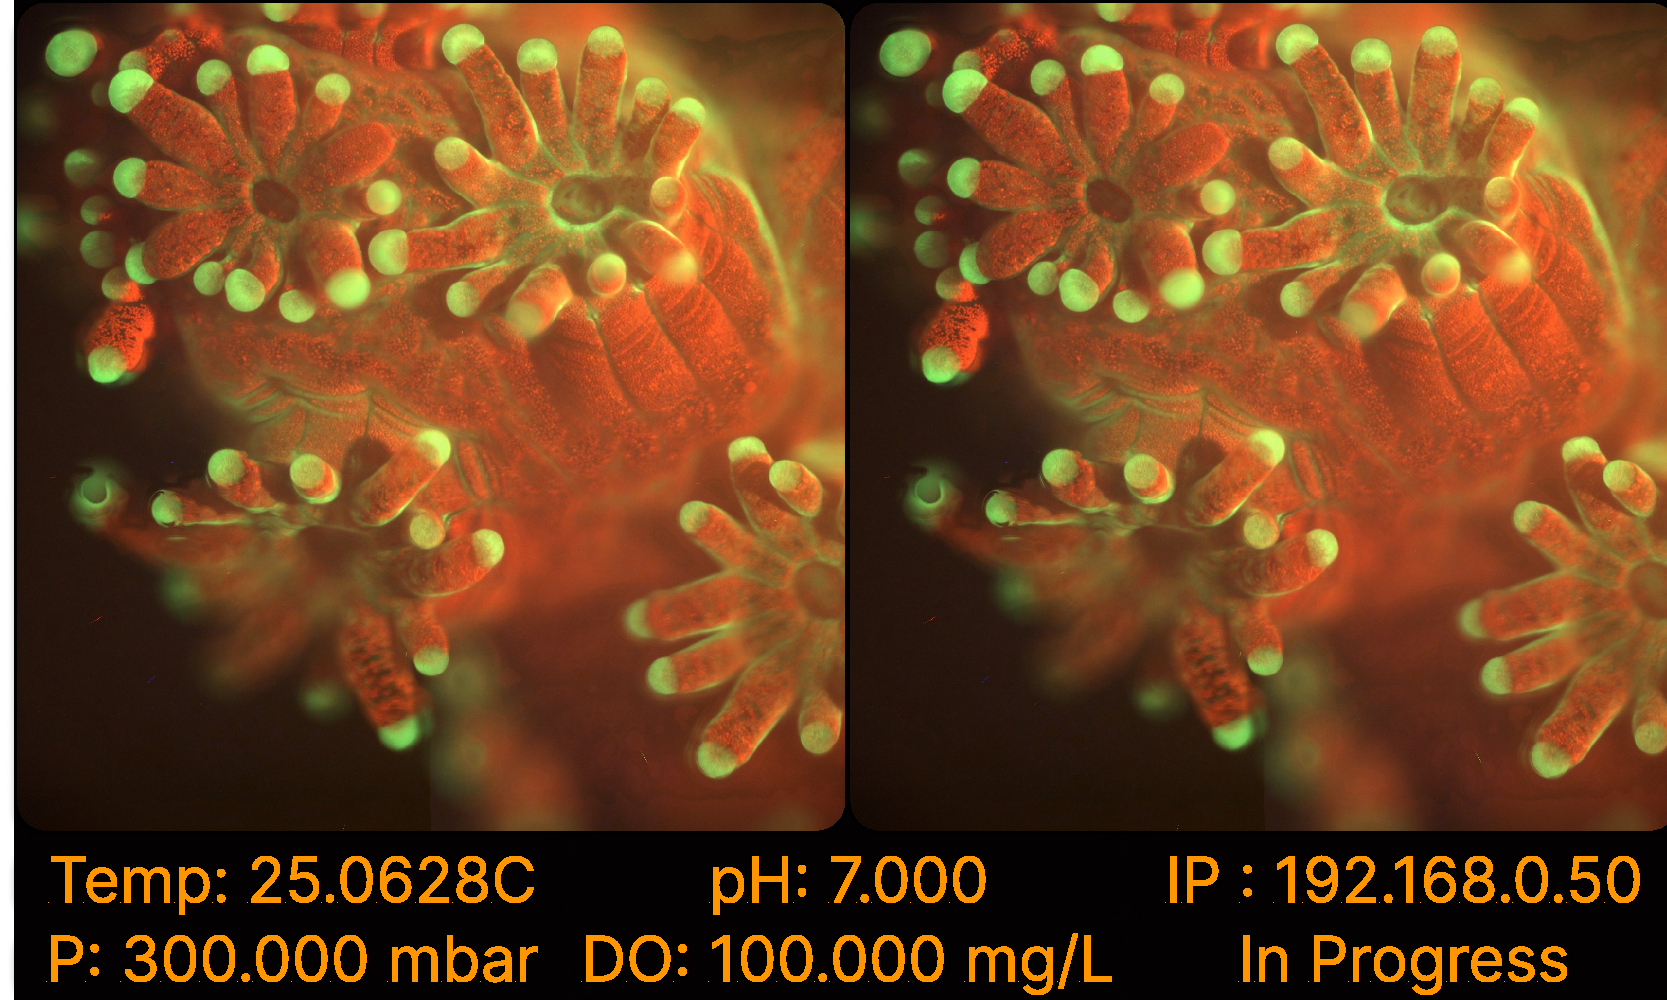
\includegraphics[page=1,height=0.7\textheight]{../../Progress_Report_Document/Appendix/Design_Documentation/User_Interface/Figures/M.O.S.I.S_UI_Design.pdf}
		\caption{Main Menu Mock-Up}
	\end{figure}
\end{frame}
\begin{frame}{M.O.S.I.S UI 2.0: Mock-ups (Study Select)}
	\begin{figure}
		\includegraphics[page=2,height=0.7\textheight]{../../Progress_Report_Document/Appendix/Design_Documentation/User_Interface/Figures/M.O.S.I.S_UI_Design.pdf}
		\caption{Main Menu Mock-Up}
	\end{figure}
\end{frame}
\begin{frame}{M.O.S.I.S UI 2.0: Class Diagram}
	\begin{figure}
		\resizebox{!}{0.7\textheight}{
			\import{../../Progress_Report_Document/Appendix/Design_Documentation/Class_Diagram/Figures/}{class_diagram}
		}
		\caption{Class Diagram}
	\end{figure}
\end{frame}
\begin{frame}{M.O.S.I.S UI 2.0: Use Case Diagram}

	\begin{figure}
		\resizebox{!}{0.7\textheight}{
			\import{../../Progress_Report_Document/Appendix/Design_Documentation/Use_Case_Diagram/Figures/}{use_case}
		}
		\caption{Use Case Diagram}
	\end{figure}
\end{frame}
\begin{frame}{M.O.S.I.S UI 2.0: Activity Diagram}
	\begin{figure}[H]
		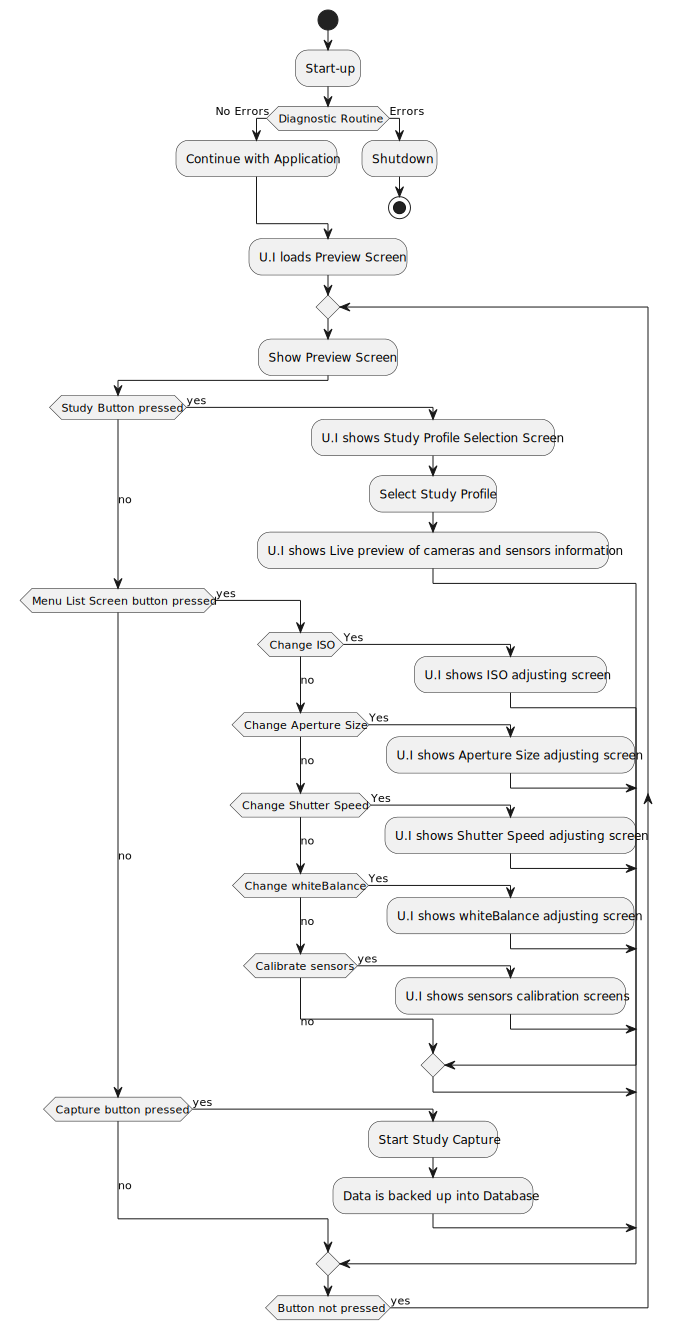
\includegraphics[page=1,height=0.7\textheight]{../../Progress_Report_Document/Appendix/Design_Documentation/Activity_Diagram/Figures/activity.pdf}
		\caption{M.O.S.I.S UI 2.0 Activity Diagram}
	\end{figure}

\end{frame}
\begin{frame}{M.O.S.I.S UI 2.0: Entity Relationship Diagram}
	\begin{figure}
		\includegraphics[page=1,height=0.7\textheight]{../../Progress_Report_Document/Appendix/Design_Documentation/ER_Diagram/Figures/ER_Diagram_MOSIS.pdf}
		\caption{ER Diagram}
	\end{figure}
\end{frame}
\subsubsection{Firmware}
\begin{frame}{Cameras: Get Snapshot}
	\begin{figure}[H]
		\begin{center}
			\resizebox{!}{0.7\textheight}{
				\import{../../Progress_Report_Document/Appendix/Design_Documentation/Firmware_Flowcharts/Figures/}{get_snapshot_flowchart}
			}
		\end{center}
		\caption{Get Snapshot Flowchart}
	\end{figure}
\end{frame}
\subsection{Project Status}
\begin{frame}{Project Status}

\end{frame}
\subsection{Deliverables}
\begin{frame}{Deliverables}

\end{frame}
\subsection{Current Budget}
\begin{frame}{Current Budget}

\end{frame}
\section{Conclusion}
\subsection{Accomplishments}
\begin{frame}{Accomplishments}

\end{frame}
\subsection{Expenditure and Budget Status}
\begin{frame}{Expenditure and Budget Status}

\end{frame}
\subsection{Future Work}
\begin{frame}{Future Work}

\end{frame}
\end{document}